\documentclass[fleqn,12pt]{article}
\usepackage{latexsym}
\usepackage[usenames]{color}
\usepackage{amssymb}
\usepackage{times}
\usepackage{graphicx}
\usepackage{caption}
\usepackage{amsmath,amsfonts,amsthm}
\usepackage{graphicx}
\usepackage{setspace}
\usepackage{pdfpages}
\usepackage{enumitem}
\usepackage{indentfirst}
\doublespacing
%\usepackage[left=2cm,top=2cm,right=2cm,footskip=20pt, bottom = 2cm,nohead]{geometry}
\usepackage{bbm}
\usepackage{nameref}
\usepackage{subfigure}
\usepackage{authblk}
\usepackage{helvet}
\usepackage{url}
\usepackage{natbib}


\renewcommand{\familydefault}{\sfdefault}

\addtolength{\oddsidemargin}{-.6in}%
\addtolength{\evensidemargin}{-.6in}%
\addtolength{\textwidth}{1.2in}%
\addtolength{\textheight}{0.4in}%
\addtolength{\topmargin}{-.8in}%


\let\oldref\ref
\renewcommand{\ref}[1]{(\oldref{#1})}

%\newcommand{\T}{^{\ensuremath{\mathsf{T}}}} % transpose
\newcommand{\T}{^{\ensuremath{\mathsf{T}}}}           % transpose
\newcommand{\mrsid}{{\sc \texttt{Mr}.~\texttt{Sid}}}
\newcommand{\argmax}{\operatornamewithlimits{argmax}}
\newcommand{\argmin}{\operatornamewithlimits{argmin}}
\newcommand{\diag}{\operatornamewithlimits{diag}}

\providecommand{\mb}[1]{\boldsymbol{#1}}
\newcommand{\bx}{\mb{x}}
\newcommand{\by}{\mb{y}}
\newcommand{\bX}{\mb{X}}
\newcommand{\bY}{\mb{Y}}



\begin{document}

\title{An M-Estimator for Reduced-Rank High-Dimensional Linear Dynamical System Identification
% A Sparse High Dimensional State-Space Model with an Application to Neuroimaging Data
}
%\author{}
\author[a]{Shaojie Chen}
\author[b]{Kai Liu}
\author[c]{Yuguang Yang}
\author[a]{Yuting Xu}
\author[d]{Seonjoo Lee}
\author[a]{Martin Lindquist}
\author[a]{Brian S. Caffo}
\author[e,f]{Joshua T. Vogelstein}
\affil[a]{\small Dept. of Biostatistics, Johns Hopkins Bloomberg School of Public Health}
\affil[b]{Dept. of Neuroscience, Johns Hopkins University}
\affil[c]{Dept. of Chemical and Biomolecular Engineering, Johns Hopkins University}
\affil[d]{Dept. of Psychiatry and Department of Biostatistics, Columbia University}
\affil[e]{Child Mind Institute}
\affil[f]{Dept. of Biomedical Enginnering and Institute for Computational Medicine, Johns Hopkins University}
\date{}
\maketitle
\section*{Abstract}
High-dimensional time-series data are becoming increasingly abundant across a wide variety of domains, spanning economics, neuroscience,  particle physics, and cosmology.  Fitting statistical models to such data, to enable parameter estimation and time-series prediction, is an important computational primitive.
Existing methods, however, are unable to cope with the high-dimensional nature of these problems, due to both computational and statistical reasons.  We mitigate both kinds of issues via proposing an M-estimator for Reduced-rank System IDentification (\mrsid). A combination of low-rank approximations, $\ell_1$ and $\ell_2$ penalties, and some numerical linear algebra tricks, yields an estimator that is computationally efficient and numerically stable.  Simulations and real data examples demonstrate the utility of this approach in a variety of problems.  In particular, we demonstrate that \mrsid~can estimate spatial filters, connectivity graphs, and time-courses from native resolution functional magnetic resonance imaging data.  Other applications and extensions are immediately available, as our approach is a generalization of the classical Kalman Filter-Smoother Expectation-Maximization algorithm.
% In the past decade functional magnetic resonance imaging (fMRI) has facilitated major advances in our understanding of human brain function. The data that arise from a standard fMRI experiment are both high dimensional and complex in nature, making statistical analysis challenging. Matrix decomposition methods, such as factor analysis, principal component analysis (PCA) and independent component analysis (ICA), are commonly used to investigate spatio-temporal patterns present in fMRI data. It can be shown that the linear time-invariant state-space model, commonly used in time series analysis, unifies this broad class of models. While state-space models have been applied to fMRI data, these applications have been limited by constraints on the amount of data that can be included in the analysis. This is primarily because analysis in modern high-dimensional settings, such as neuroimaging, parameter estimation is challenging. This issue is addressed by introducing a penalized state-space model that applies $\ell_1$ and $\ell_2$ penalties to model coefficients. In addition, an Expectation-Maximization algorithm is provided that allows for efficient estimation of the model parameters. To illustrate our approach, we apply it to fMRI data measured over the motor cortex.
\\
\textbf{\emph{keywords}: state-space model, parameter estimation, sparsity, imaging processing, fMRI}
%\newpage
\section{Introduction}

%\begin{itemize}
%\item proposed a penalized linear dynamical system model (\mrsid)
%\item designed an expectation-maximization algorithm to solve the proposed model
%\item used the model for neuroimage data analysis and explored the primary motor cortex of human brain
%\end{itemize}
High-dimensional time-series data are becoming increasingly abundant across a wide variety of domains, spanning economics \citep{Johansen1988}, neuroscience \citep{Friston2003a},   and cosmology \citep{Xie2013a}.
Fitting statistical models to such data, to enable parameter estimation and time-series prediction, is an important computational primitive.
Linear dynamical systems (LDS) models are amongst the most popular and powerful, because of their intuitive nature and ease of implementation \citep{Kalman1963}.   The famous Kalman Filter Smoother is one of the most popular and powerful tool for time-series prediction with an LDS, given known parameters \citep{Kalman1960a}.
In practive, however, for many LDSs, the parameters are unknown, and must be estimated, a process often called \emph{system identification} in this domain \citep{Ljung1998}.  To date, there does not exist, to our knowledge, a methodology that provides parameter estimates and predictions from ultrahigh-dimensional time-series data (for example, $p > 10$,$000$).

The challenges associated high-dimensional time-series estimation and prediction are multifold.  First, na\"{i}vely such models include dense $p \times p$ matrices, which often are too large even to store, and much too large to invert in memory.  For large sparse matrices, recently, several efforts to invert them using a series of computational tricks are promising, though still extremely computationally expensive  \citep{Hsieh2013, Banerjee2013a}.
Second, estimators behave poorly, due to numerical instability issues.
Reduced rank LDS models reduce the number of latent dimensions, and therefore partially address this problem \citep{CHEN1989}.  However, without further constraints, the dimensionality of the latent states must be so small as to significantly decrease the predictive capacity of the resulting model.  Third, even after addressing these problems, the time to compute all the necessary quantities can be overly burdensome. Distributed memory implementations, such as using Spark, might help to overcome this problem, but it would at additional costs and set-up burden, as it would require a Spark cluster \citep{Zaharia2010}.

We address all three of these issues with our M-estimator for Reduced-rank  System IDentification (\mrsid).  By assuming the dimensionality of the latent state space is small (reduced rank), relative to the ambient, or observed, space dimensionality, we can significantly improve computational tractability and estimation accuracy. By further penalizing the estimators, with $\ell_1$ and/or $\ell_2$ penalties, utilizing prior knowledge on the structure of the parameters, we gain further estimation accuracy in this high-dimensional but relatively low-sample size regime.  Finally, by employing several numerical linear algebra tricks, we can bring the computational burden down significantly.

These three techniques together enable us to obtain highly accurate estimates in a variety of simulation settings.  \mrsid~is, in fact, a generalization of the now classic Baum-Welch expectation maximization algorithm, commonly used for system identification in much lower dimensional linear dynamical systems \citep{rabiner1989tutorial}. We numerically show that the hyper-parameters can be selected minimizing prediction error on held-out data.  Finally, we use \mrsid~to estimate functional connectomes from motor cortex.  \mrsid~enables us to estimate the regions, rather than imposing some prior parcellation on the data, as well as estimate sparse connectivity between regions.  \mrsid~reliably estimates these connectomes, as well as predicts the held-out time-series data.  To our knowledge, this is the first time anybody has been able to estimate partitions and functional connectomes directly from the high-dimensional data, with a single unified approach.  To enable extensions, generalizations, and additional applications, the functions and code for generating each of the figures is freely available on Github. (referred to as the Git Repo in following sections) %from \url{https://github.com/shachen/PLDS/} (referred to as the PLDS Git Repo in following sections).



\section{The Model}

In statistical data analysis, one often encounter some observed variables, as well as some unobserved latent variables, which we denote as $\bY=(\by_1,\ldots,\by_T)$ and $\bX=(\bx_1,\ldots,\bx_T)$ respectively. By the Bayesian rule, the joint probability of $\bY$ and $\bX$ is $P(\bX,\bY)=P(\bY|\bX) P(\bX)$. The conditional distribution $P(\mb{Y}|\mb{X})$ and prior $P(\mb{X})$ can both be represented as a product of marginals:
\begin{equation*}
\begin{aligned}
P(\mb{Y}|\mb{X}) &= \prod_{t=1}^T P(\by_t | \by_0,\ldots,\by_{t-1}, \bx_0,\ldots,\bx_{t-1}), \\
P(\bX) &= P(\bx_0) \prod_{t=1}^T P(\bx_t | \bx_0,\ldots,\bx_{t-1}).
\end{aligned}
\end{equation*}

The generic time-invariant state-space model (SSM) makes the following simplifying assumptions
\begin{equation*}
\begin{aligned}
P(\by_t | \by_0,\ldots,\by_{t-1}, \bx_0,\ldots,\bx_t)  &\approx P(\by_t | \bx_t), \\
P(\bx_t | \bx_0,\ldots,\bx_{t-1}) &\approx P(\bx_t | \bx_{t-1}).
\end{aligned}
\end{equation*}

A linear dynamical system (LDS) further assumes that both of the above terms are linear Gaussian functions, which, when written as an iterative random process, yields the standard matrix update rules:
% or LDS, further assumes that the latent variables follow a vector autoregressive model and the observed variables are normally distributed given the latent variables, as follows:
\begin{equation*}
\begin{aligned}
&\bx_{t+1}=A\bx_t+\mathbf{w}_t, \quad \mathbf{w}_t\sim N(\mathbf{0},Q),\quad \bx_0 \sim N(\mathbf{\pi}_0,V_0)\\
&\by_t=C\bx_t+\mathbf{v}_t,\qquad \mathbf{v}_t\sim N(\mathbf{0},R),
\end{aligned}
\end{equation*}
where $A$ is a $d\times d$ state transition matrix and $C$ is a $p \times d$ generative matrix. $\bx_t$ is a $d\times 1$ vector and $\by_t$ is a $p\times 1$ vector.
% The sequence of vectors $\bY=(\by_1,\ldots,\by_T)$ are the observed data and $\bX=(\bx_1,\ldots,\bx_T)$ represent the unknown hidden states.
The output noise covariance $R$ is $p\times p$, while the state noise covariance $Q$ is $d\times d$. Initial state mean $\mathbf{\pi}_0$ is $d\times 1$ and covariance $V_0$ is $d \times d$.

The model can be thought as the continuous version of the hidden Markov model (HMM), where the columns of $C$ stands for the hidden states. The difference is that in this model, what one observe at time $t$ is not a single state, but a linear combination of multiple states. $\bx_t$ keeps the weights in the linear combination. $A$ matrix is the analogy of the state transition matrix, which describe how the weights $\bx_t$ evolve over time. Another difference is that LDS contains two white noise terms, which are captured by the $Q$ and $R$ matrices.

Without applying further constraints, the LDS model itself is unidentifiable. Three basic constraints are introduced to make it identifiable:
\vspace*{-3mm}
\begin{equation*}\label{eq:constraints1}
\begin{aligned}
&\text{Constraint 1: }Q \text{ is the identity matrix}\\
&\text{\text{Constraint 2:} the ordering of the columns of } C \text{ is fixed based on their norms}\\
&\text{Constraint 3: } V_0=\mathbf{0}
\end{aligned}
\end{equation*}
Note that the first two constraints follow directly from Roweis and Ghahramani (1999) \citep{roweis1999unifying}.

The logic for Constraint 1 is as follows. Since covariance matrix $Q$ is symmetric and positive semidefinite, it can be decomposed as $E\Lambda E^T$, where $E$ is a rotation matrix of eigenvectors and $\Lambda$ is a diagonal matrix of eigenvalues. Then for any model whose $Q$ is not the identity matrix, one can always generate an equivalent model using a new state vector $\mathbf{z}=\Lambda^{-1/2} E^T \bx$, with $A_{\mathbf{z}}=(\Lambda^{-1/2}E^T)A(E\Lambda^{1/2})$ and $C_{\mathbf{z}}=C(E\Lambda^{1/2})$. The covariance of new vector $\mathbf{z}$ is the identity matrix, i.e., $Q_{\mathbf{z}}=\mathbf{I}$. Thus one can constrain $Q=\mathbf{I}$ without loss of generality.

For Constraint 2, the components of the state vector can be arbitrarily reordered; this corresponds to swapping the columns of $C$ and $A$. Therefore,the order of the columns of matrix $C$ must be fixed. We follow Roweis and Ghahramani and choose the order by decreasing the norms of columns of $C$.

Additionally, $V_0$ is set to zero, meaning the starting state $\bx_0=\mathbf{\pi}_0$ is an unknown constant instead of a random variable. This is reasonable, as in many applications, there is often only one single chain of time series observed. To estimate $V_0$ accurately, multiple series of observations are required.
%%While it is not necessary to constrain $\mathbf{\pi_0}=\mathbf{0}$, one can do so as the observed data can always be centered. When we center the observed data, we implicitly enforced $\mathbf{\pi_0}=\mathbf{0}$.

The following three constraints are further applied to achieve a more useful model.
\vspace*{-3mm}
\begin{equation*}\label{eqn:constraints2}
\begin{aligned}
&\text{Constraint 4: }R\text{ is a diagonal matrix}\\
&\text{Constraint 5: }A\text{ is sparse}\\
&\text{Constraint 6: }C\text{ has smooth columns}
\end{aligned}
\end{equation*}

Consider the case where the observed data are high dimensional, the $R$ matrix can be very large. One can not accurately estimate the many free parameters in $R$ with a limited amount of observations. Therefore, some constraints on $R$ will help with inferential accuracy, by virtue of significantly reducing variance while not adding too much bias. In the simplest case, $R$ is set to an identity matrix or its multiple. More generally, one can also constrain $R$ to be diagonal. In the static model with no temporal dynamics, a diagonal $R$ is equivalent to the generic Factor Analysis method, while multiples of the identity $R$ matrix lead to Principal Component Analysis (PCA) \citep{roweis1999unifying}.

$A$ matrix is the transition matrix of the hidden states. In many applications, it is desirable for $A$ to be sparse. In this work, an $\ell_1$ penalty on $A$ is used to impose the sparsity constraints. In the applications that follow, $A$ is a central construct of interest representing a so-called connectivity graph, and the graph is expected to be sparse.

Similarly, in many applications, one wants the columns of $C$ to be smooth. For example, in neuroimaging data analysis, each column of $C$ can be a signal in the brain. Having the signals spatially smooth can help extract meaningful information from the noisy neuroimaging data. In this context, an $\ell_2$ penalty on columns of $C$ is used to enforce smoothness.

With all those constraints, the model becomes:
\begin{equation}\label{eq:model0}
\begin{aligned}
	&\bx_{t+1}=A\bx_{t}+\mathbf{w}_t, \quad \mathbf{w}_t\sim N(\mathbf{0},\mathbf{I}),\quad \bx_0 = \mathbf{\pi}_0\\
	&\by_t=C\bx_t+\mathbf{v}_t,\qquad \mathbf{v}_t\sim N(\mathbf{0},R).
\end{aligned}
\end{equation}

where $A$ is a sparse matrix and $C$ has smooth columns.
% For notational convenience, a sequence of $T$ output vectors $(\by_1,\ldots,\by_T)$ is denoted by $\bY$. %; a subsequence $(\by_{t_0},\by_{t_0 + 1},\ldots,\by_{t_1})$ by $\bY_{t_0}^{t_1}$.
% Similarly for the latent states.
% In addition, l
Let $\theta =\{A,C,R,\mathbf{\pi}_0\}$ represents all unknown parameters and $P(\bX,\bY)$ be the full likelihood, then combing model \ref{eq:model0} and the constraints on $A$ and $C$ leads us to an optimization problem
\begin{equation}\label{eqn:penaltylik}
\hat{\theta}=\argmin_{\substack{\theta}}\left\{-\log P_\theta(\bX,\bY)+\lambda_1\|A\|_1+\lambda_2\|C\|_2^2\right\}
\end{equation}
where $\lambda_1$ and $\lambda_2$ are tuning parameters and $\|\centerdot\|_p$ represents the $p$-norm of a vector. Equivalently, this problem has the following dual form
\begin{equation*}\label{eqn:penaltylikdual}
\begin{aligned}
&\text{minimize}&\left\{-\log P_\theta(\bX,\bY)\right\}&\\
&\text{subject to: }
& \alpha\|A\|_1+ (1-\alpha)\|C\|_2^2 \leq t \text{ for some }t; &\\
&& A\in \mathcal{A}_{d\times d},\ C \in \mathcal{C}_{p \times d}, R \in \mathcal{R}_{p\times p}, \pi_0 \in \mathcal{\pi}_{d\times 1}.&
\end{aligned}
\end{equation*}
where $\alpha = \frac{\lambda_1}{\lambda_1 + \lambda_2}$. $\mathcal{A}_{d\times d}$ and $\mathcal{C}_{p \times d}$ are $d\times d$ and $p \times d$ dimensional matrix spaces respectively. $\mathcal{R}_{p \times p}$ is the $p \times p$ diagonal matrix space and $\mathcal{\pi}_{d\times 1}$ is the $d$ dimensional vector space.
\section{Parameter Estimation}
Parameter estimation requires solving optimization problem \ref{eqn:penaltylik}: given only one observed sequence (or multiple sequences in some applications) of outputs $\bY=(\by_1,\ldots,\by_T)$, find the parameters $\theta=\{A,C,R,\mathbf{\pi}_0\}$ that maximize the likelihood of observations.

Parameter estimation for LDS has been investigated extensively in statistics, machine learning, control theory and signal processing research. For example, in machine learning, exact and variational inference algorithms for general Bayesian networks can be applied to LDS. In control theory, the corresponding area of study is known as system identification.

Specifically, one way to search for the maximum likelihood estimation (MLE) is through iterative methods such as expectation maximization (EM) \citep{shumway1982approach}. The EM algorithm for a standard LDS is detailed in Zoubin and Geoffrey (1996) \citep{ghahramani1996parameter}. An alternative is to use subspace identification methods such as N4SID and PCA-ID, which give asymptotically unbiased closed-form solutions \citep{van1994n4sid,doretto2003dynamic}. In practice, determining an initial solution with subspace identification and then refining it with EM is an effective approach \citep{bootslearning}.

However, the above approaches are not directly applicable to optimization problem \ref{eqn:penaltylik} due to the introduced penalty terms. We therefore developed a novel algorithm called M-estimation for Reduced rank System IDentification (\mrsid), as detailed in the following.

By the chain rule, the full likelihood is
\begin{equation*}\label{eqn:likelihood}
\begin{aligned}
P(\bX,\bY)&=P(\bY|\bX) P(\bX)\\
&= P(\bx_0)\prod\limits_{t=1}^{T}P(\bx_t|\bx_{t-1})\prod\limits_{t=1}^{T} P(\by_t|\bx_t)=\prod\limits_{t=1}^{T}P(\bx_t|\bx_{t-1})\prod\limits_{t=1}^{T} P(\by_t|\bx_t)\mathbbm{1}_{\mathbf{\pi}_0}(\bx_0)
\end{aligned}
\end{equation*}
where $\mathbbm{1}_{\mathbf{\pi}_0}(\bx_0)$ is the indicator function. Conditional likelihoods are
\begin{equation*}\label{eqn:condlik}
\begin{aligned}
P(\by_t|\bx_t)&= (2\pi)^{-\frac{p}{2}}|R|^{-\frac{1}{2}}\  \text{exp}\left\{-\frac{1}{2}[\by_t-C\bx_t]^{\T}R^{-1}[\by_t-C\bx_t]\right\}\\
P(\bx_t|\bx_{t-1})
%%&=\text{exp}\left\{-\frac{1}{2}[\mathbf{x_t}-A\mathbf{x_{t-1}}]^{\T}Q^{-1}[\mathbf{x_t}-A\mathbf{x_{t-1}}]\right\}(2\pi)^{-d/2}|Q|^{-1/2}\\
&=(2\pi)^{-\frac{d}{2}}\  \text{exp}\left\{-\frac{1}{2}[\bx_t-A\bx_{t-1}]^{\T}[\bx_t-A\bx_{t-1}]\right\}.
\end{aligned}
\end{equation*}

Then the log-likelihood, after dropping a constant, is just a sum of quadratic terms
%\begin{equation}\label{eqn: loglik}
%\begin{split}
%\text{log} P(\bX,\bY)=&-\sum\limits_{t=1}^{T}\big(\frac{1}{2}[\mathbf{y_t}-C\mathbf{x_t}]^{\prime}R^{-1}[\mathbf{y_t}-C\mathbf{x_t}]\big)-\frac{T}{2}\text{log}|R|\\
%&-\sum\limits_{t=1}^{T}\big(\frac{1}{2}[\mathbf{x_t}-A\mathbf{x_{t-1}}]^{\prime}\mathbf{Q}^{-1}[\mathbf{x_t}-A\mathbf{x_{t-1}}]\big)-\frac{T}{2}\text{log}|\mathbf{Q}|\\
%&-\frac{1}{2}[\mathbf{x_0}-\mathbf{\pi_0}]^{\prime}\mathbf{V_0}^{-1}[\mathbf{x_0}-\mathbf{\pi_0}]-\frac{1}{2}\text{log}|\mathbf{V_0}|-\frac{T(p+d+1)}{2}\text{log}2\pi
%\end{split}
%\end{equation}
\begin{equation}\label{eqn:loglik}
\begin{split}
\log  P(\bX,\bY)=&-\sum\limits_{t=1}^{T}\big(\frac{1}{2}[\by_t-C\bx_t]^{\T}R^{-1}[\by_t-C\bx_t]\big)-\frac{T}{2}\text{log}|R|\\
&-\sum\limits_{t=1}^{T}\big(\frac{1}{2}[\bx_t-A\bx_{t-1}]^{\T}[\bx_t-A\bx_{t-1}]\big)-\frac{T}{2}\text{log}|\mathbf{I}|+ \text{log}(\mathbbm{1}_{\mathbf{\pi}_0}(\bx_0)).
\end{split}
\end{equation}

Replace $\log  P(\bX,\bY)$ in problem \ref{eqn:penaltylik} with equation \ref{eqn:loglik}, one gets
\begin{equation}\label{eqn:penaltylik2}
\begin{split}
\hat{\theta}=\argmin_{\substack{\theta}}\biggl\{&\sum\limits_{t=1}^{T}\big(\frac{1}{2}[\by_t-C\bx_t]^{\T}R^{-1}[\by_t-C\bx_t]\big)-\frac{T}{2}\text{log}|R|\\
&+\sum\limits_{t=1}^{T}\big(\frac{1}{2}[\bx_t-A\bx_{t-1}]^{\T}[\bx_t-A\bx_{t-1}]\big)-\frac{T}{2}\text{log}|\mathbf{I}| - \text{log}(\mathbbm{1}_{\mathbf{\pi}_0}(\bx_0))\\
&+\lambda_1\|A\|_1+\lambda_2\|C\|_2^2\biggr\}.
\end{split}
\end{equation}

Denote the target function in the curly braces  as $\mathbf{\Phi}(\theta,\bY,\bX)$, then $\mathbf{\Phi}$ can be optimized with \mrsid, a generalized Expectation-Maximization (EM) algorithm.

\subsection{E Step}
The E step of EM requires computation of the expected log likelihood, $\Gamma = E[\log P(\bX,\bY|\bY)]$. This quantity depends on three expectations: $E[\bx_t|\bY]$, $E[\bx_t\bx_t^{\T}|\bY]$ and $E[\bx_t\bx_{t-1}^{\T}|\bY]$. For simplicity, we denote their finite sample estimators by:
\begin{equation}\label{eq:expecs}
%\begin{aligned}
\hat{\bx}_t \equiv E[\mathbf{x_t}|\bY],\  \hat{P}_t  \equiv E[\bx_t\bx_t^{\T}|\bY],\  \hat{P}_{t,t-1}  \equiv E[\bx_t\bx_{t-1}^{\T}|\bY].
%\end{aligned}
\end{equation}

Expectations \ref{eq:expecs} are estimated with a Kalman filter/smoother, which is detailed in the Appendix on the Git Repo. Notice that all expectations are taken with respect to the current estimations of parameters.
\subsection{M Step}
Each of the parameters in $\theta =\{A,C,R,\mathbf{\pi}_0\}$ is estimated by taking the corresponding partial derivatives of $\mathbf{\Phi}(\theta,\bY,\bx)$, setting to zero and solving.

Denote estimations from previous step as $\theta^{\text{old}} =\{A^{\text{old}},C^{\text{old}},R^{\text{old}},\mathbf{\pi}_0^{\text{old}}\}$ and current estimations as $\theta^{\text{new}} =\{A^{\text{new}},C^{\text{new}},R^{\text{new}},\mathbf{\pi}_0^{\text{new}}\}$. Estimation for $R$ matrix has closed form,
\begin{equation}\label{eq:updateR}
\begin{aligned}
\frac{\partial \mathbf{\Phi}}{\partial R^{-1}} &= \frac{T}{2}R - \sum\limits_{t=1}^T\bigl(\frac{1}{2}\by_t\by_t^{\T} - C\hat{\bx}_t\by_t^{\T}+\frac{1}{2}C\hat{P}_tC^{\T}\bigr) =0 \\
\implies R &= \frac{1}{T}\sum\limits_{t=1}^{T}(\by_t\by_t^{\T}-C^{\text{new}}\hat{\bx}_t\by_t^{\T})\\
\implies R^{\text{new}} &= \diag \biggl\{\frac{1}{T}\sum\limits_{t=1}^{T}(\by_t\by_t^{\T}-C\hat{\bx}_t\by_t^{\T})\biggr\}
\end{aligned}
\end{equation}
In the bottom line, $\diag$ extracts only the diagonal of the in-bracket term, as we constrain $R$ to be diagonal in Constraint 4.

Estimation for $\mathbf{\pi}_0$ has closed form. The relevant term $\log(\mathbbm{1}_{\mathbf{\pi}_0}(\hat{\bx}_0))$ is minimized only when $\mathbf{\pi}_0^{\text{new}} = \hat{\bx}_0$.

Estimation for $C$ matrix also has closed form. Terms involving $C$ in equation \ref{eqn:penaltylik2} are
\begin{equation*}
f_{\lambda_2}(C;\bX,\bY) = \sum\limits_{t=1}^{T}\left(\frac{1}{2}[\by_t-C\bx_t]^{\T}R^{-1}[\by_t-C\bx_t]\right)+\lambda_2 \|C\|_2.
\end{equation*}

In $f_{\lambda_2}(C;\bX,\bY)$, $C$ is a matrix, to simplify notation and optimization, we vectorized it to a vector $\mathbf{c}$ following the methods of \citet{turlach2005simultaneous}. A closed form solution for $\mathbf{c}$, $\mathbf{c}^{\text{new}}$, is given by the Tikhonov regularization \citep{tikhonov1943stability}. Rearrange the elements in $\mathbf{c}^{\text{new}}$, one gets an estimation of matrix $C$. That is,
\begin{equation}\label{eq:updatec}
C^{\text{new}} =\text{Rearrange } \mathbf{c}^{\text{new}}
\end{equation}
The details of estimating $C$ can be found in the Git Repo Appendix.

Now let's look at matrix $A$. Terms involving $A$ in equation \ref{eqn:penaltylik2} are,
\begin{equation*}
f_{\lambda_1}(A;\bX,\bY) = \sum\limits_{t=1}^{T}\big(\frac{1}{2}[\bx_t-A\bx_{t-1}]^{\T}[\bx_t-A\bx_{t-1}]\big)+\lambda_1 \|A\|_1.
\end{equation*}

Similar to what we have done to $C$, $f_{\lambda_1}(A;\bX,\bY)$ is equivalent to
\begin{equation*}
f_{\lambda_1}(A;\bX,\bY) =  \|\mathbf{z}  - \mathbf{Za}\|_2^2 + \lambda_1\|\mathbf{a}\|_1.
\end{equation*}
where $\mathbf{z}$ is a $Td \times 1$ vector from rearranging $\bX$ and $\mathbf{Z}$ is a block diagonal matrix with diagonal component $Z^{\T} =(\bx_0,\ldots,\bx_{T-1})^{\T}$.


$f_{\lambda_1}(A;\bX,\bY)$ does not have closed form solution due to the $\ell_1$ term. Fortunately, it can be solved numerically with a Fast Iterative Shrinkage-Thresholding Algorithm (FISTA) \citep{beck2009fast}. The FISTA algorithm is detailed in the Appendix on the Git Repo.

With FISTA, matrix $A$ can be updated:
\begin{equation}\label{eq:updatea}
A^{\text{new}} = \text{FISTA}(\|\mathbf{Z}^{\T}\mathbf{a}^{\text{old}} -\mathbf{z}\|_2^2,\quad \lambda_1)
\end{equation}

\subsection{Initialization}\label{sec:initial}
$R$ matrix is initialized as the identify matrix, while $\mathbf{\pi}_0$ as $\mathbf{0}$ vector. For $A$ and $C$, denote $\bY = \left[\mathbf{y_1},\cdots,\mathbf{y_T}\right]$, a $p\times T$ matrix, then the singular value decomposition (SVD) of $\bY$ is $\bY = \mathbf{UDV^{\T}} \approx \mathbf{U}_{p \times d} \mathbf{D}_{d \times d} \mathbf{V}_{d \times T}^{\T} =\mathbf{U}_{p\times d}\bX_{d \times T}$, where $\mathbf{U}_{p \times d}$ is the first $d$ columns of $\mathbf{U}$ and $\mathbf{D}_{d\times d}$ is the upper left block of $\mathbf{D}$. This notation also applies to $\mathbf{V}^{\T}_{d \times T}$.
%\begin{equation}\label{eq:initial}
%    \bY = \mathbf{UDV^{\T}} \approx \mathbf{U}_{p \times d} \mathbf{D}_{d \times d} \mathbf{V}_{d \times T}^{\T} =\mathbf{U}_{p\times d}\bX_{d \times T}
%\end{equation}
$C$ is then initialzed as $\mathbf{U}_{p\times d}$, while the columns of $\bX_{d \times T}$ are used as input for a vector autoregressive (VAR) model to estimate the initial value for $A$.

Combining the initialization, E-step and M-step, a complete EM algorithm for \mrsid~is addressed in Table \oldref{tab:em}. Notice that all the terms involving $\bX$ in the M-step are approximated with the conditional expectations calculated in E-step.\\
\begin{table}
\captionof{table}{The Complete EM Algorithm}
\label{tab:em}
\begin{tabular}{l}
\hline
\textbf{Algorithm } EM Algorithm for \mrsid\\
\hline
\textbf{M Step}\\
%1. Replace all $\bx_t$ in \eqref{eqn: penaltylik2} with E$(\bx_t|\{\by_t\}_1^T)$ from E step\\
1. $R^{\text{new}}=\diag\biggl\{\frac{1}{T}\sum\limits_{t=1}^{T}(\by_t\by_t^{\T}-C^{\text{old}} \hat{\bx}_t\by_t^{\T})\biggr\}$, as in equation \ref{eq:updateR}\\
2. $\mathbf{\pi}_0^{\text{new}}=\hat{\bx}_0$\\
3. Update $C^{\text{new}}$, as in equation \ref{eq:updatec}\\
4. Update $A^{\text{new}}$ with FISTA, as in equation \ref{eq:updatea}\\
5. Stop when difference between estimations from this step and previous step\\
  $\quad$ is less than tolerance or maximum number of iterations reached.\\
\hline
\textbf{E Step}\\
0. Initialize $\theta =\{A,C,R,\mathbf{\pi}_0\}$ as in Section \oldref{sec:initial}, if first loop\\
1. Update the expectations in \ref{eq:expecs} with the Kalman filter smoother\\
\hline
\end{tabular}
\end{table}


\subsection{Improving Computational Efficiency}
The major factors that affect the efficiency and scalability of the above EM algorithm involve the storage and computations of covariance matrix $R$. The following computational techniques are utilized to make the code highly efficient and scalable.

First, a sparse matrix is used to represent R. When dimension $p$ gets higher, the size of $R$ increase quadratically, which will easily exceed the memory capacity of a computer.  Fortunately, with Constraint 4, $R$ is sparse and can be represented with a sparse matrix.

In addition, the diagonal is directly calculated instead of first calculating the full matrix $R$ in M step.

Finally, in E-step, the term $K_t=V_t^{t-1}C^{\T}(CV_t^{t-1}C^{\T}+R)^{-1}$ involves the inverse of a large square matrix of $p$ by $p$, which might be intractable. The Woodbury Matrix Identity is employed to turn a high dimensional matrix inverse to low dimensional one: $(CV_t^{t-1}C^{\T}+R)^{-1} = R^{-1} - R^{-1}C[(V_t^{t-1})^{-1} + C^{\T}R^{-1}C]^{-1}C^{\T}R^{-1}$.

Also note that quantities like $R^{-1}$ and $C^{\T}R^{-1}C$ can be pre-computed and reused throughout the E step. With the above three techniques, the EM algorithm can scale to very high dimensions in terms of $p$, $d$ and $T$, without causing any computational issues.


\section{Simulations}
\subsection{Simulation Setup}
\label{sec:simsetup}
Two simulations of different dimensions are performed to demonstrate parameter estimations, computational efficiency and predicting ability of \mrsid.

In the low dimensional setting, $p = 300$, $d = 10$ and $T = 100$. $A$ is first generated from a random matrix, then elements with small absolute values are truncated to zero to make it sparse. After that a multiple of the identity matrix is added to $A$. Finally $A$ is scaled to make sure its eigenvalues fall within $[-1,1]$, thus avoiding diverging time series. Matrix $C$ is generated as follows. Each column contains random samples from a standard Gaussian. Then each column is sorted in ascending order. Covariance $Q$ is the identity matrix and covariance $R$ is a multiple of the identity matrix. Initial state $\mathbf{\pi}_0 = \mathbf{0}$ is a zero vector. Pseudocode for data generation can be found in the Appendix on Git Repo.

In the high-dimensional setting, $p = 10000$, $d = 30$ and $T = 100$. The parameter are generated in a the same manner.

To evaluate the accuracy of estimations, we elect to define the distance between two matrices $A$ and $B$ as
%\begin{equation}\label{eq:distance}
%d( A,B) = -\log(\frac{1}{n}\max_{P\in P(n)} \text{ Tr}\bigl(P\times C_{A,B}\bigr))
%\end{equation}
\begin{equation}\label{eq:distance}
d(A,B) = \argmin_{P\in P(n)}\left\{\log\bigl[\frac{n}{\text{\footnotesize Trace}(P\times C_{A,B})}\bigr]\right\}.
\end{equation}
where $C_{A,B}$ is the correlation matrix between columns of A and B, $P(n)$ is a collection of all the permutation matrices of order n and $P$ is a permutation matrix.

As a result of its definition, $d(A,B)$ is invariant to the scales of $A$ and $B$. It is also invariant to a permutation of columns of either matrix. The calculation of $d(A,B)$ is a linear assignment problem and can be solved in polynomial time with the Hungarian algorithm \citep{kuhn1955hungarian}.


\subsection{Parameter Estimation}
\label{sec:lowdsim}

Both the standard LDS and the penalized LDS are applied to the simulation data. Since $A$ is sparse and $C$ is smooth, we expect the penalized algorithms to yield better estimations with properly chosen penalty size. When the penalties are approaching 0, the penalized algorithm should converge to the non-penalized algorithm. In addition, when the penalties are too big or too small compared to the optimal values, estimations might be less accurate.

A sequence of tuning parameters $\lambda_C$ are tested, ranging from $10^{-6}$ to $10^4$. $\lambda_A = k \lambda_C$ is set to increase proportionally with $\lambda_C$, where $k$ is a constant.

Estimation accuracies are plotted against penalty size $\lambda_C$ in Figure \oldref{fig:low-high-d-sim}. Results from LDS and \mrsid~are overlayed in one plot for comparison. As the figure shows, \mrsid~converges to the LDS when the penalties are approaching zero. Estimation accuracies first increase with penalty size and then decrease due to over-shrinkage.

\begin{figure}
\centering
\subfigure[Low dimensional setting]{%
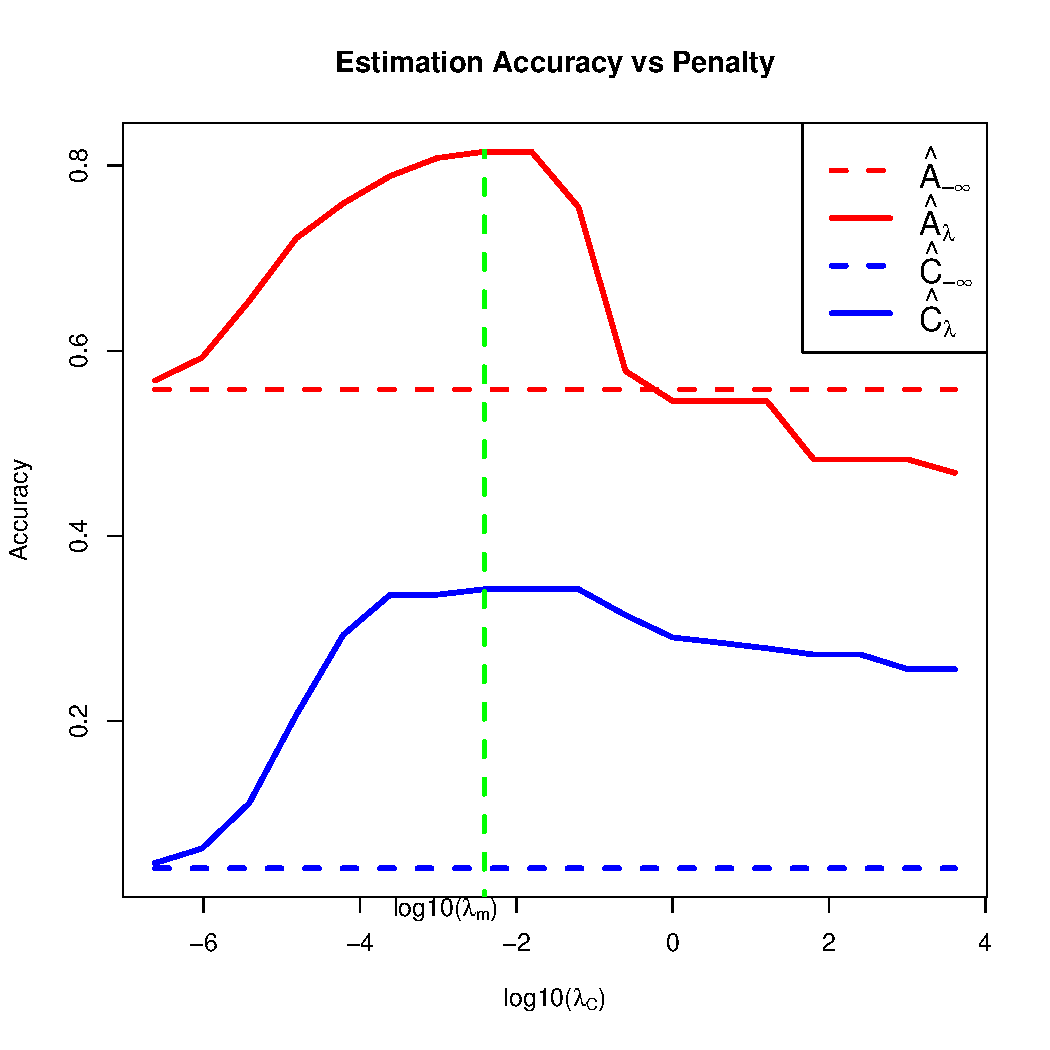
\includegraphics[scale=.43]{./figures/low-d-simulation.pdf}
}
\subfigure[High dimensional setting]{%
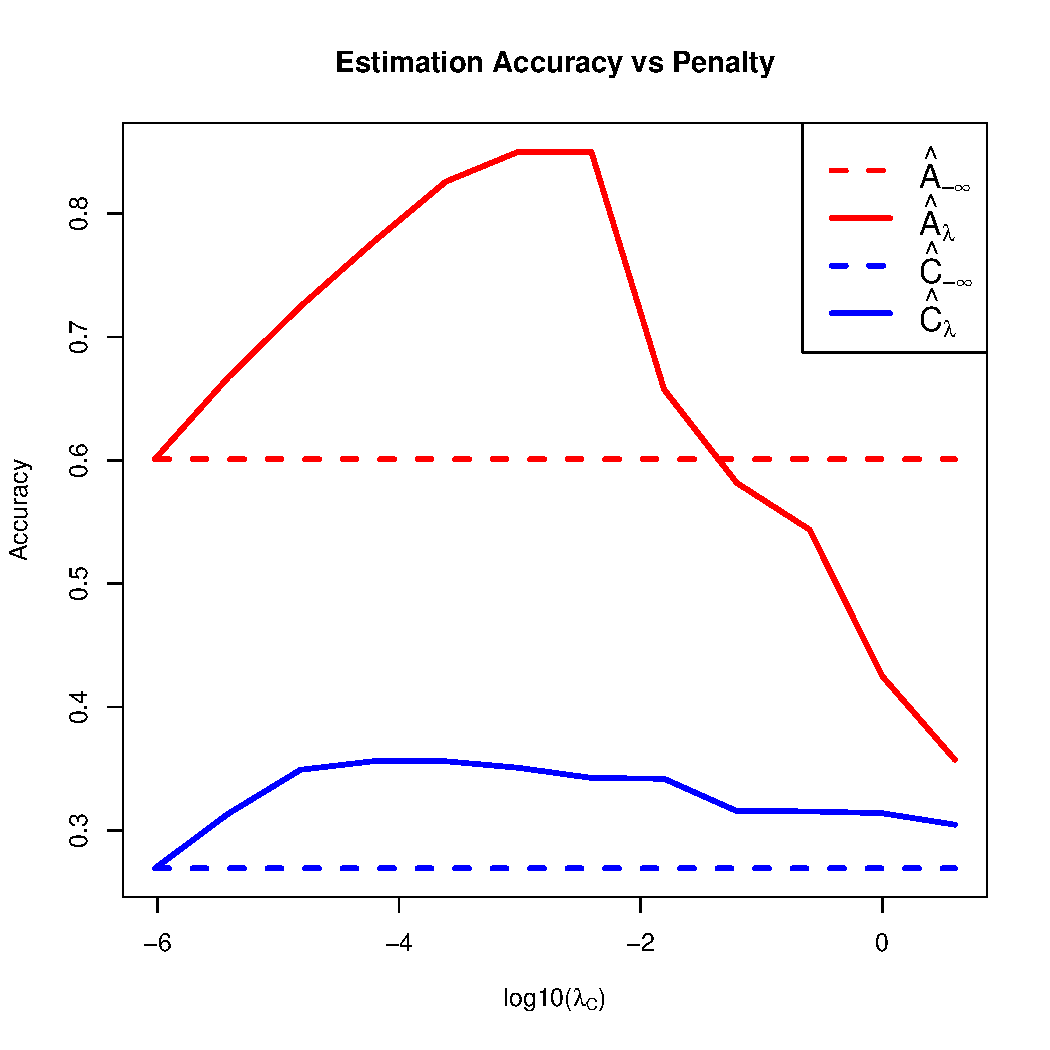
\includegraphics[scale=.43]{./figures/high-d-simulation.pdf}
}
\caption{$x$ axis is tuning parameter $\lambda_C$ under log scale and $y$ axis is the distance between truth and estimations; $\lambda_A$ is increasing proportionally with $\lambda_C$. One can see that in both the low dimensional and hight dimensional setting, estimation accuracies for $A$ and $C$ first increase then decrease as penalty increases.}
\label{fig:low-high-d-sim}
\end{figure}


As a concrete example, estimations from both methods are compared to the true values of parameters in Figure \oldref{fig:heatmap}. One can see that true values in each column of $C$ matrix are decreasing smoothly. $\hat{C}_{\lambda_m}$, which is estimated with optimal penalties $\lambda_C = \lambda_m$ and $\lambda_A = k\lambda_m$, shows similar pattern. In terms of $A$, the true value is sparse with many $0$ (blue) values. \mrsid~estimation $\hat{A}_{\lambda_m}$ is also sparse, denoted by the off-diagonal 0 (blue) values. However, LDS estimation $\hat{A}_{\lambda_{-\infty}}$ is not sparse, with many positive (yellow and red) off-diagonal values.
\begin{figure}
 \centering
 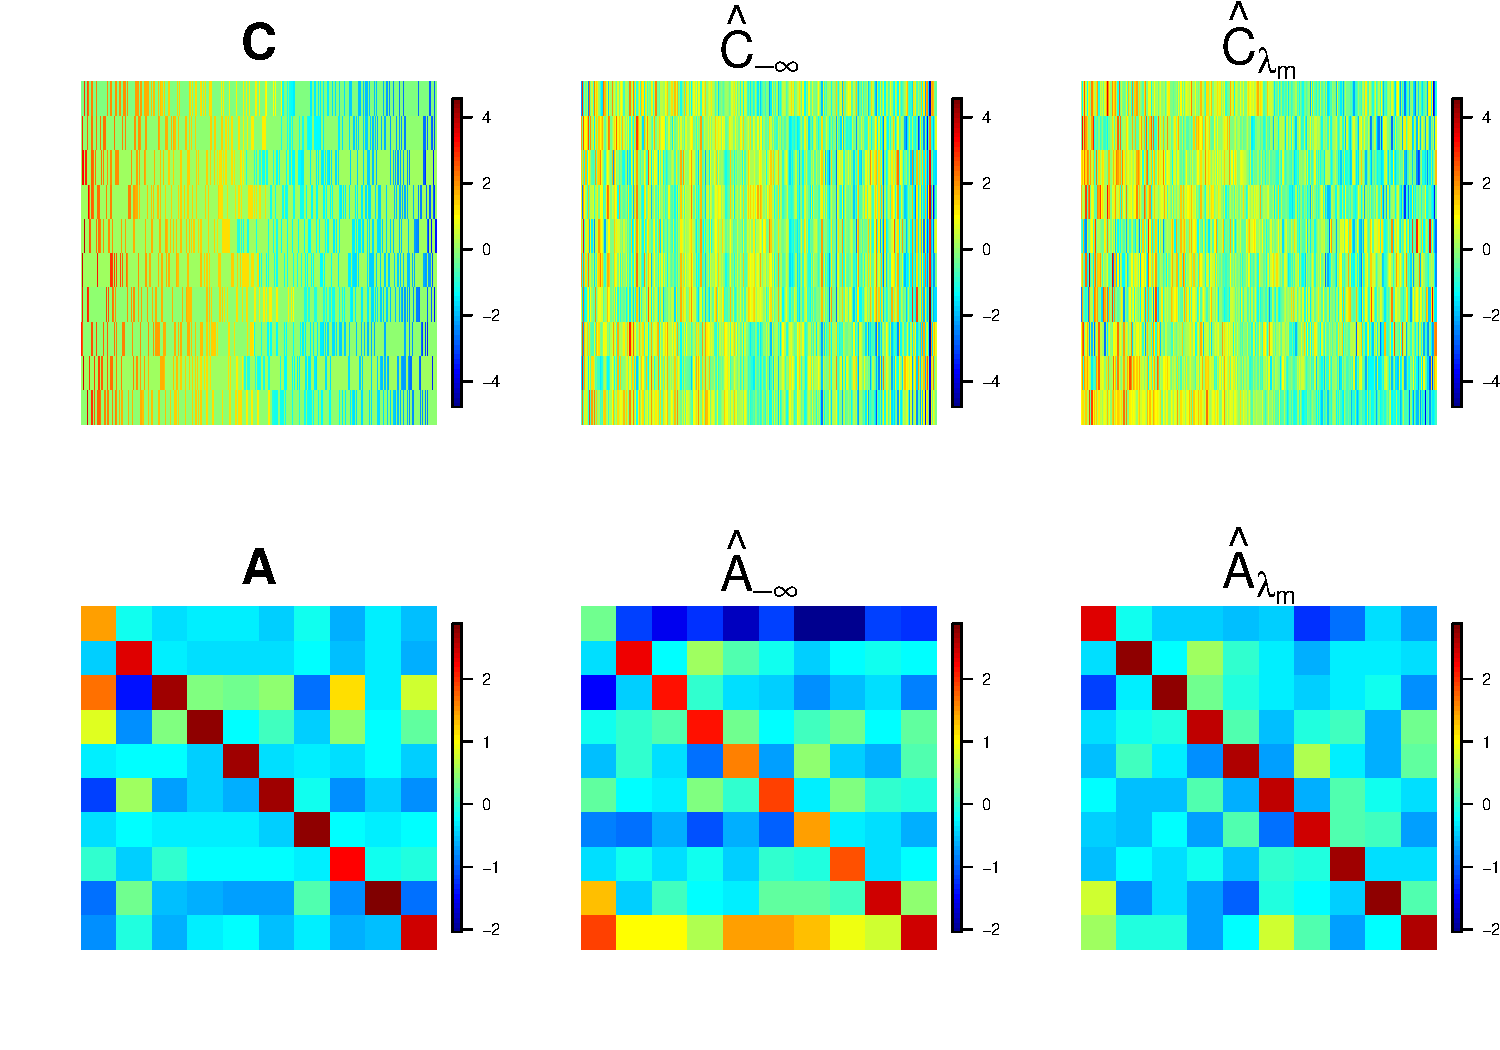
\includegraphics[scale=.6]{./figures/heatmap-figure-1}
 \captionof{figure}{Row 1: $C$ truth; non-penalized estimation of $C$; optimally penalized estimation of $C$. Row 2: $A$ truth; non-penalized estimation of $A$; optimally penalized estimation of $A$.}
 \label{fig:heatmap}
\end{figure}

In addition to the improved estimation accuracy, the proposed algorithm is also computational efficient and highly scalable. As a demonstration, the running times of multiple simulation scenarios are summarized in Table \oldref{tab:runningTime}. When both $p$ and $d$ are high dimensional, the algorithm can still solve the problem in a reasonable time.
\begin{table}
\centering
\captionof{table}{\mrsid~Running Time}
\label{tab:runningTime}
\begin{tabular}{c|ccccc}
\hline\hline
$p$ & 100 & 1000 & 10000 & 100000 & 100000\\
\hline
$d$ & 10 & 30 & 50 & 100 & 500 \\
\hline
$T$ & 100 & 300 & 500 & 1000 & 1000 \\
\hline
Time (min)& 0.07 & 0.30  & 5.15 & 111.38 & 1127.18 \\
\hline\hline
\end{tabular}
\end{table}
\subsection{Making Predictions}
Another perspective when considering \mrsid~is its ability to make predictions. When the parameters $\mathbf{\theta}$ and the latent state $x_T$ are estimated, one can first use $x_T$ to predict $x_{T+1}$ and then use $x_{T+1}$ to predict $y_{T+1}$. Similarly, more predictions $y_{T+2},\ldots, y_{T+k}$ can be made. As shown above, properly chosen penalties give good estimations. With good estimations, one can expect accurate predictions. This idea is demonstrated with a simulation. The same data are used as in Section \oldref{sec:simsetup}. $80\%$ of the data are used for estimation, while the other $20\%$ used for prediction. Correlations between predictions and true signals are used as a measure of accuracy. The prediction accuracy over penalty size is plotted in Figure \oldref{fig:estpredaccuracy}.

\begin{figure}
\centering
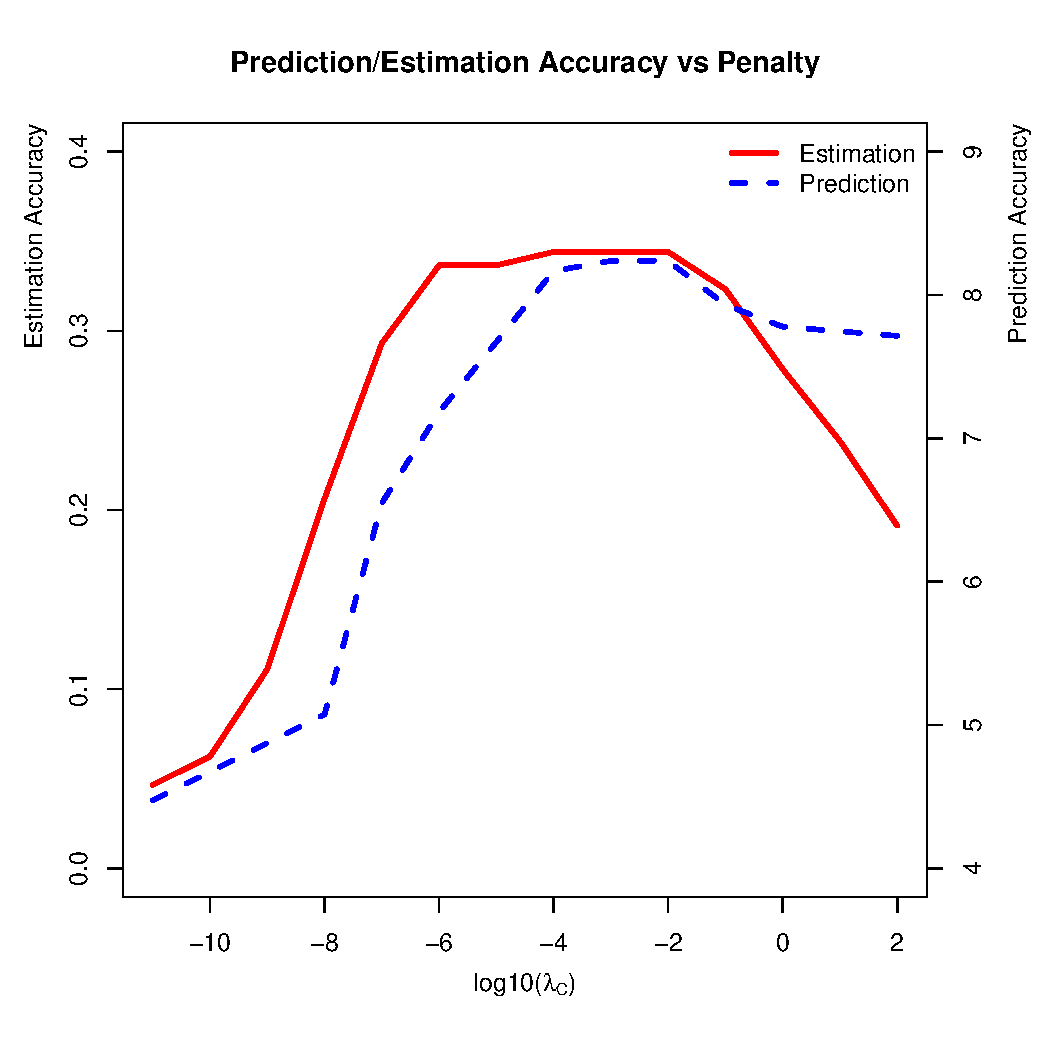
\includegraphics[scale=0.46]{./figures/est-pred-accuracy.pdf}
\captionof{figure}{Estimation and prediction accuracies. $x$-axis is the penalty size under $\log$ scale. $y$-axis represents the estimation and prediction accuracies. One see that the penalty which yields the most accurate estimation also gives the best predictions.}
\label{fig:estpredaccuracy}
\end{figure}

From the plots one can see, the prediction accuracy first improves then drops when the penalties increase. The prediction accuracy peaks when the penalty coefficient $\lambda_A$ and $\lambda_C$ are around $10^{-3}$. This makes good sense as the same $(\lambda_A,\lambda_C)$ pair also gives the best estimations of $A$ and $C$, as in Figure \oldref{fig:low-high-d-sim}. The latter observation provides us a way to pick tuning parameters in real applications: one can use a collection of tuning parameter pairs $(\lambda_A,\lambda_C)$ for estimations and then predictions, the pair that gives most accurate predictions is picked. This trick is used in application Section \oldref{sec:application}.

\section{Application}
\label{sec:application}

\subsection{Data and Motivation}

\mrsid~is applied to two datasets in this section: the Kirby 21 data and the Human Connectome Project (HCP) data.

The Kirby 21 data are resting-state fMRI scans acquired at the FM Kirby Research Center at the Kennedy Krieger Institute, Johns Hopkins University \citep{landman2011multi}. Twenty-one healthy volunteers with no history of neurological disease each underwent two separate resting state fMRI sessions on the same scanner: a 3T MR scanner utilizing a body coil with a 2D echoplanar (EPI) sequence and eight channel phased array SENSitivity Encoding (SENSE; factor of 2) with the following parameters: TR 2s; 3mm$\times$3mm in plane resolution; slice gap 1mm; and total imaging time of 7 minutes and 14 seconds. The imaging data are first preprocessed with FSL, a comprehensive library of analysis tools for fMRI, MRI and DTI brain imaging data \citep{smith2004advances}. FSL is used for spatial smoothing with Gaussian kernel. Then \mrsid~is applied on the smoothed data.

The Human Connectome Project (HCP) is a systematic effort to map macroscopic human brain circuits and their relationship to behavior in a large population of healthy adults \citep{van2013wu,moeller2010multiband,feinberg2010multiplexed}. MR scanning includes four imaging modalities, acquired at high resolutions: structural MRI, resting-state fMRI (rfMRI), task fMRI (tfMRI), and diffusion MRI (dMRI). All 1200 subjects are scanned using all four of these modalities on a customized 3 T scanner.  All scans consist of 1200 time points. A comprehensive introduction of the dataset is given by \cite{van2013wu}.

For both datasets, the motor cortex, which contains $p=7396$ voxels is analyzed instead of the whole brain.

Extensive research has been done to analyze the above datasets. Methods such as PCA and ICA (independent component analysis) have been applied to get spatial decompositions of the brain, as well as the functional connectivity among the decomposed regions. Motivated by these research, we are applying \mrsid~to the Kirby 21 data and wish to get a spatial decomposition and a connectivity graph at the same time. It would also be very helpful, especially in medical sciences, if one can predict the brain activity from already-collected data. Therefore, as a second application, \mrsid~ is applied to the HCP data to predict brain activities.


\subsection{Results}

\mrsid~is first applied to the Kirby 21 data.

When applied to fMRI data, the model has very good interpretability. Each $\by_t$ is a snapshot of brain activity at time $t$. The columns of $C$ are interpreted as time-invariant brain ``point spread functions''. At each time point, the observed brain image, $\by_t$, is a linear mixture of latent co-assemblies of neural activity  $\bx_t$. Matrix $A$ describes how $\bx_t$ evolves over time. $A$ is a directed graph if one treats each neural assembly as a vertex. Each neural assembly is spatially smooth, and connectivity across them are empirically sparse. This naturally fits into the sparsity and smoothness assumptions of \mrsid.


In this application, the number of voxels, $p = 7396$ and number of scans, $T = 210$. Tuning parameters: $\lambda_A = \lambda_C = 10^{-5}$. Number of latent states, $d = 11$. Max number of iterations for EM and the regularized subproblems are both 30 steps.

To pick optimal penalty size, different combinations of $\lambda_A$ and $\lambda_C$, where $\lambda_A = \lambda_C$ are tried. The values range from $10^{-10}$ to $10^{4}$. Then the estimations from each combination are used to make predictions. The combination that gives the best prediction is used. One can also use a grid of combinations to search for even better penalties.

To determine the number of latent states, the profile likelihood method proposed by Zhu et al. \citep{zhu2006automatic} is adopted. The method assumes eigenvalues of the data matrix come from a mixed Gaussian and use profile likelihood to pick the optimal number of latent states. Apply the method to all four scans, the numbers of latent states are 11, 6, 14 and 15 respectively. Their average, $d=11$, is used.

First look at estimations of the $A$ matrix. Let $A_{12}$ stands for the estimated $A$ matrix for the second scan of subject one. Similar logic applies to $A_{11}, A_{21}$, $A_{22}$ and $C$ matrices. These matrices contain subject-specific information. There are $6$ different pairs among the $4$ matrices - intuitively, the pair $(A_{11},A_{12})$ and $(A_{21},A_{22})$ should have the highest similarity, as each comes from two scans of the same subject. This idea is validated by Table \oldref{tab:similarity} and Figure \oldref{fig:matsim}, which summarize similarities among the  $4$ matrices. The distance measure in Equation \ref{eq:distance} is used. Another permutation-invariant measure of similarity, the Amari error \citep{amari1996new}, is also provided. The Amari error between matrices $A$ and $\hat{A}$ is defined as: $E(A,\hat{A}) = \sum\limits_{i=1}^n(\sum\limits_{j=1}^n\frac{|p_{ij}|}{\max_k |p_{ik}|}-1) + \sum\limits_{j=1}^n(\sum\limits_{i=1}^n\frac{|p_{ij}|}{\max_k|p_{kj}|}-1)$, where $P =(p_{ij})=A^{-1}\hat{A}$. Notice a smaller $d(A,B)$ or Amari error means higher similarity.

\begin{table}
\centering
\captionof{table}{Similarities Among Estimated $A$ Matrices}
\label{tab:similarity}
\begin{tabular}{c|cccc}
\hline
$d(\cdot,\cdot)$(Amari Error) & $A_{11}$&$A_{12}$ & $A_{21}$&$A_{22}$ \\
\hline
$A_{11}$ & $0$ &  &  &\\
$A_{12}$ & $\mathbf{0.076(0.88)}$& $0$ & &\\
$A_{21}$ & $0.105(1.05)$ & $0.095(1.08)$  & $0$ &\\
$A_{22}$ & $0.095(1.02)$ & $0.095(1.09)$ & $\mathbf{0.085(0.98)}$ & $0$ \\
\hline
\end{tabular}
\end{table}

\begin{center}
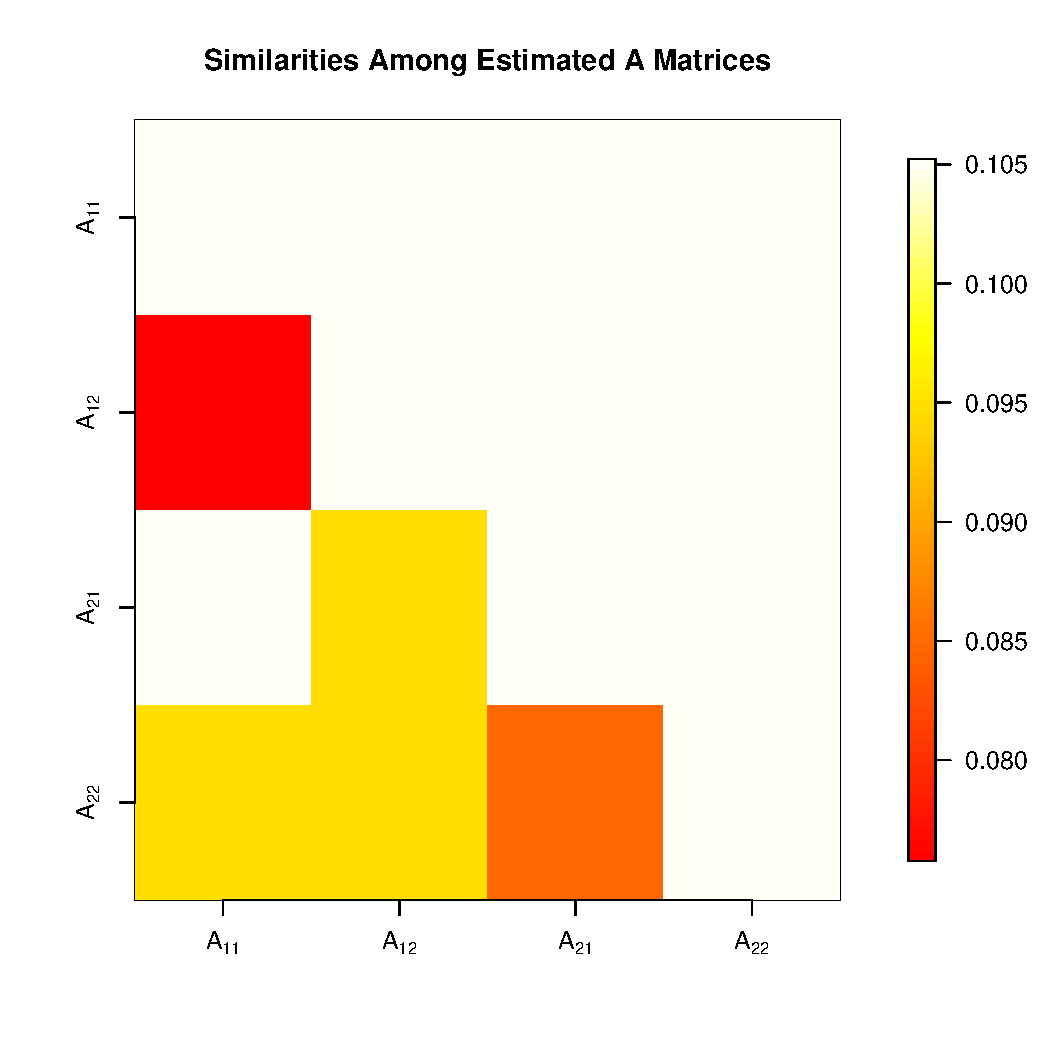
\includegraphics[scale=.4]{./figures/A-matrices-similarity.pdf}
\captionof{figure}{Similarities among the four estimated $A$ matrices. The distance $d(\cdot,\cdot)$ is used in this figure. The two red/orange off-diagonal pixels has the minimum distances, which correspond to the pairs of $(A_{11},A_{12})$ and $(A_{21},A_{22})$ respectively. With this similarity map, one can tell which two scans are from the same subject.}
\label{fig:matsim}
\end{center}

Next let's turn to the $C$ matrix. 3D renderings of the columns of $C_{11}$ are shown in Figure \oldref{fig:3d} (after thresholding). These regions are comparable to existing parcellations of the mortor cortex. As an example, the blue region in Figure \oldref{fig:3d} accurately matches the dorselmedical (DM) parcel of the five-region parcellation proposed by Nebel MB et al. \citep{nebel2014disruption}.
\begin{center}
\[
\begin{array}{lll}
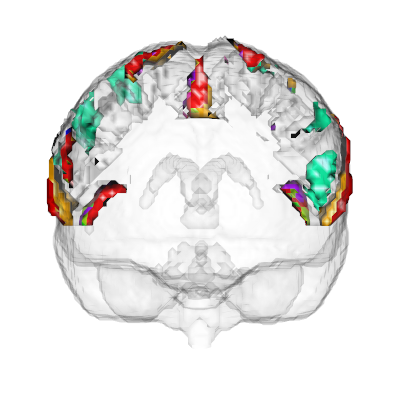
\includegraphics[scale = 0.36]{./figures/view1.png} & 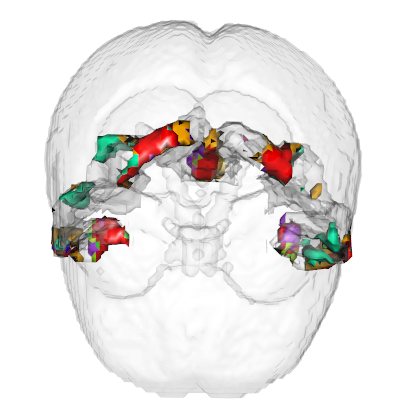
\includegraphics[scale = 0.33]{./figures/view2.png} & 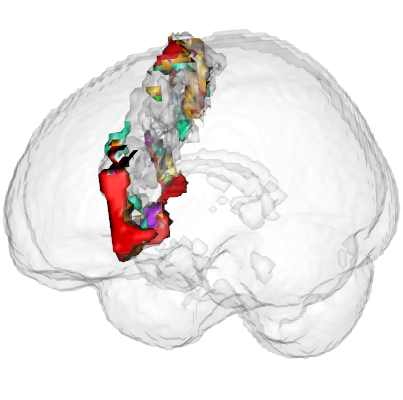
\includegraphics[scale = 0.33]{./figures/view3.png}
%\includegraphics[scale = 0.21]{view1-26.png} & \includegraphics[scale = 0.21]{view2-26.png} & \includegraphics[scale = 0.21]{view3-26.png}
\end{array}
\]
\captionof{figure}{3D rendering of columns of matrix $C_{11}$: estimation for the first scan of subject one.}
\label{fig:3d}
\end{center}

As a summary, \mrsid~ gives a spatial decomposition of the motor cortex, as well as the sparse connectivity among the decomposed regions. The connectivity graph contains subject-specific information and can correctly group scans by subject. The decomposed regions are spatially smooth and are comparable to existing parcellations of the motor cortex.

As a second application, \mrsid~is applied to the HCP data to predict brain activities.

Using the profile likelihood method, $d=149$ is picked. HCP data has $T=1200$ time points. The first $N = 1000$ are used as training data, while the rest are used for test.

\mrsid~is used to predict brain activity from training data. As a comparison, the SVD method in Section \oldref{sec:initial} is also tried. Both methods are first used for parameter estimations, then the estimated parameters are fed into equations \ref{eq:model0} to make $k$-step ahead predictions. Pseudocode for $k$-step ahead predictions is given in Appendix on Git Repo.

The prediction accuracies are shown in Figure \oldref{fig:predaccy} (left panel). One can see \mrsid~algorithm is giving significantly better predictions for the first 150 predictions compared to the SVD method. Considering the SVD method is also used to intialize \mrsid~algorithm, this observation shows that \mrsid~algorithm improves estimation accuracy significantly on top of the SVD method. Another observation is, \mrsid~algorithm's performance get worse when one predicts into the ``long" future ($>150$ steps). This is reasonable because the prediction errors from each step will accumulate and yields deteriorating predictions as the number of steps increase.

\begin{center}
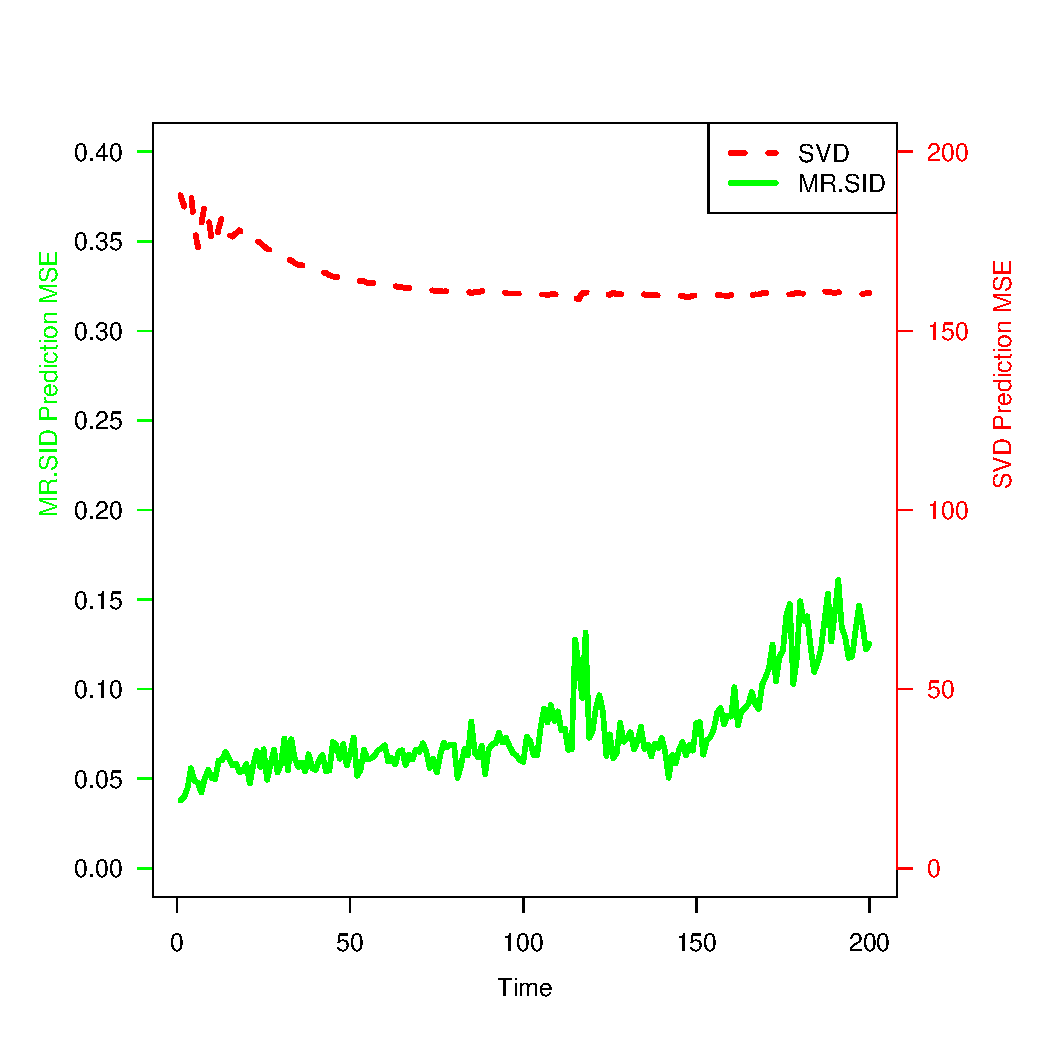
\includegraphics[scale=0.45]{./figures/hcp_pred_accy.pdf}
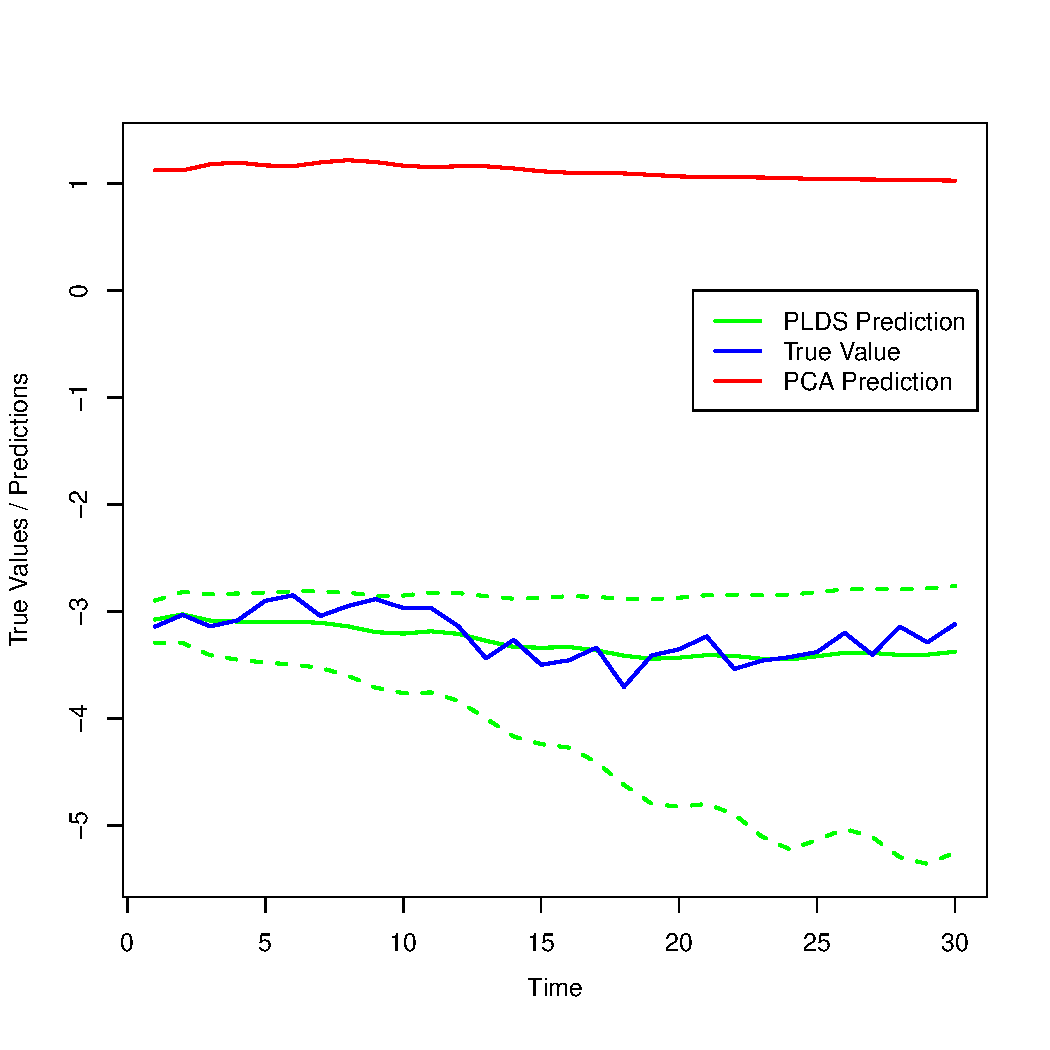
\includegraphics[scale=0.45]{./figures/newSampleTS.pdf}
\captionof{figure}{Prediction accuracies comparison on HCP data.
\emph{Left:} The mean squared error (MSE) is used as the accuracy measure.
\emph{Right:} Sample time series plot. The dotted green curve stands for the $60\%$ confidence band given by \mrsid~model. The true time series is averaged signals from a subsample of voxels. The predictions are also averaged over the same subsample. The confidence band is estimated based on the covariance matrix of these voxels. A subsample of 20 voxels are picked in this experiment to avoid big covariance matrices calculation. All values are log-scaled for plotting purpose.
}
\label{fig:predaccy}
\end{center}


A sample plot of the true time series and predicted values are shown in Figure \oldref{fig:predaccy} (right panel). We see that \mrsid~is giving more accurate predictions and the true signal lies in the confidence band giving by \mrsid~model. Another observation is that the confidence band is getting wider as we predict into the future, which is a result of the accumulated errors.


\section{Discussion}

By applying the proposed model to fMRI scans of the motor cortex of healthy adults, we identify limited sub-regions (networks) from the motor cortex. A statistical procedure should be further developed to match these regions to existing parcellations of the motor cortex.

In the future, this work could be extended in two important directions. First, assumptions on the covariance structures in the observation equation could be generalized. Prior knowledge could be incorporated to covariance $R$ \citep{allen2014generalized}. The general rule is that $R$ should be general enough to be flexible while sufficiently restricted to make the model useful. A lot of other platforms such as tridiagnol and upper triangular could also be considered. Mohammad et al. have discussed the impact of auto correlation on functional connectivity, which also provides us a direction for extension \citep{arbabshirani2014impact}.

Finally, the work can also be extended on the application side. Currently, only data from a few subjects are analyzed. As a next step, the model can be extended to a group version and be used to analyze more subjects. In addition, $A$ matrix estimated by \mrsid~is a potential candidate as a measure of fMRI scan reproducibility.


%\bibliographystyle{ieeetr}
\bibliographystyle{Chicago}
\bibliography{reference}
\end{document}
